%-------------------------------%
% Template modify from Alexander Soen's Student Assignment Template
%https://www.overleaf.com/latex/templates/student-assignment-template/sjkprrdkmphg
%-------------------------------%

\documentclass[a4paper]{article}
\usepackage{student}
\usepackage{float}

% Metadata
\date{\today}
\setmodule{Assignment 2 Report}
\setterm{114-1 (Fall 2025)}

%-------------------------------%
% Other details
% TODO: Fill the information
%-------------------------------%
\title{Reinforcement Learning}
\setmembername{Ivan Chang} % In English
\setmemberuid{B13901165}
%-------------------------------%
% Add / Delete commands and packages
% TODO: Add / Delete here as you need
%-------------------------------%
\usepackage{amsmath,amssymb,bm}

\newcommand{\KL}{\mathrm{KL}}
\newcommand{\R}{\mathbb{R}}
\newcommand{\E}{\mathbb{E}}
\newcommand{\T}{\top}

\newcommand{\expdist}[2]{%
        \normalfont{\textsc{Exp}}(#1, #2)%
    }
\newcommand{\expparam}{\bm \lambda}
\newcommand{\Expparam}{\bm \Lambda}
\newcommand{\natparam}{\bm \eta}
\newcommand{\Natparam}{\bm H}
\newcommand{\sufstat}{\bm u}

% Main document
\begin{document}
    % Add header
    \header{}

    % Use `answer` environment to add solutions
    % \begin{answer}[Question 1] for example starts an environment formatted
    % for Question 1
    \begin{answer}[Q1. Run Monte-Carlo prediction and TD(0) prediction for 50 seeds. Compare the resulting values with the GT values. Discuss the variance and bias. ]
        \textbf{Description:} \\
        During this session, I implemented both Monte-Carlo  and TD(0) for prediction tasks. I ran the experiments for over 50 different seeds
        and compared the results with the ground truth values. The bias and variance are shown in the figures below.

        \begin{figure}[H]
            \centering
            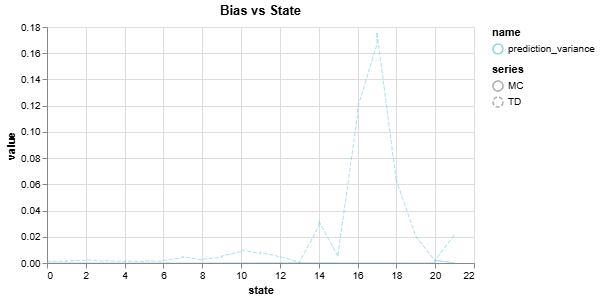
\includegraphics[width=0.5\textwidth]{Myimages/prediction_bias.png}
            \caption{Bias vs state}
            \label{fig:prediction_bias}
        \end{figure}

        \begin{figure}[H]
            \centering
            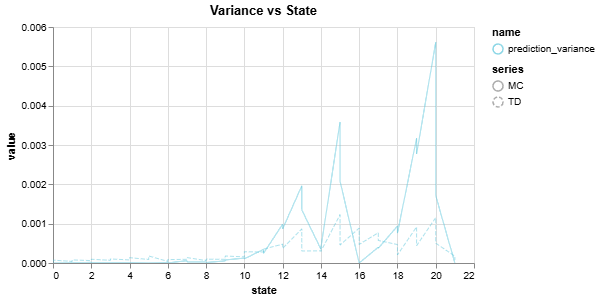
\includegraphics[width=0.5\textwidth]{Myimages/prediction_variance.png}
            \caption{Variance vs state}
            \label{fig:prediction_variance}
        \end{figure}
        \textbf{Analysis:} \\
        \begin{enumerate}
            \item \textbf{Bias:} In the bias plot, we can observe that the bias for Monte-carlo is nearly zero across all states,
            while the bias for TD(0) is significantly higher, especially in the middle states. The reason behind this effect is that Monte-Carlo use the full return to update the value function,
            which provides an unbiased estimate of the true value(the value function will converge to the true value in the long run).
            On the other hand, TD(0) uses bootstrapping to update the value function, which induces bias since we are using an estimate to update another estimate.
            \item \textbf{Variance:} The variance plot shows that Monte-Carlo has a much higher variance compared to TD(0). The reason for this is that Monte-Carlo uses the full return to update the value function,which 
            will take in all the randomness in the episode. In contrast, TD(0) only uses the one-step return to update the value function, which reduces the variance since it only considers the immediate reward.
            and the randomness is only from the next state.
            \item \textbf{Overall Comparison:} In summary, the results shows a trade-off between bias and variance for Monte-Carlo and TD(0).
            That is the reason why $TD(\lambda)$ is developed to balance the bias-variance trade-off by using n-step returns.
        \end{enumerate}
        
       
    \end{answer}
    \begin{answer}[Q2. Discuss and plot learning curves under $\epsilon$ values of $(0.1, 0.2, 0.3, 0.4)$ on MC, SARSA, and Q-Learning ]
        \textbf{Description:} \\
        During this session, I implemented Monte-Carlo, SARSA, and Q-Learning for control tasks. I ran the experiments for over 4 different $\epsilon$ values
        and compared the learning curves. The learning curves are shown in the figures below.
        \begin{figure}[H]
            \centering
            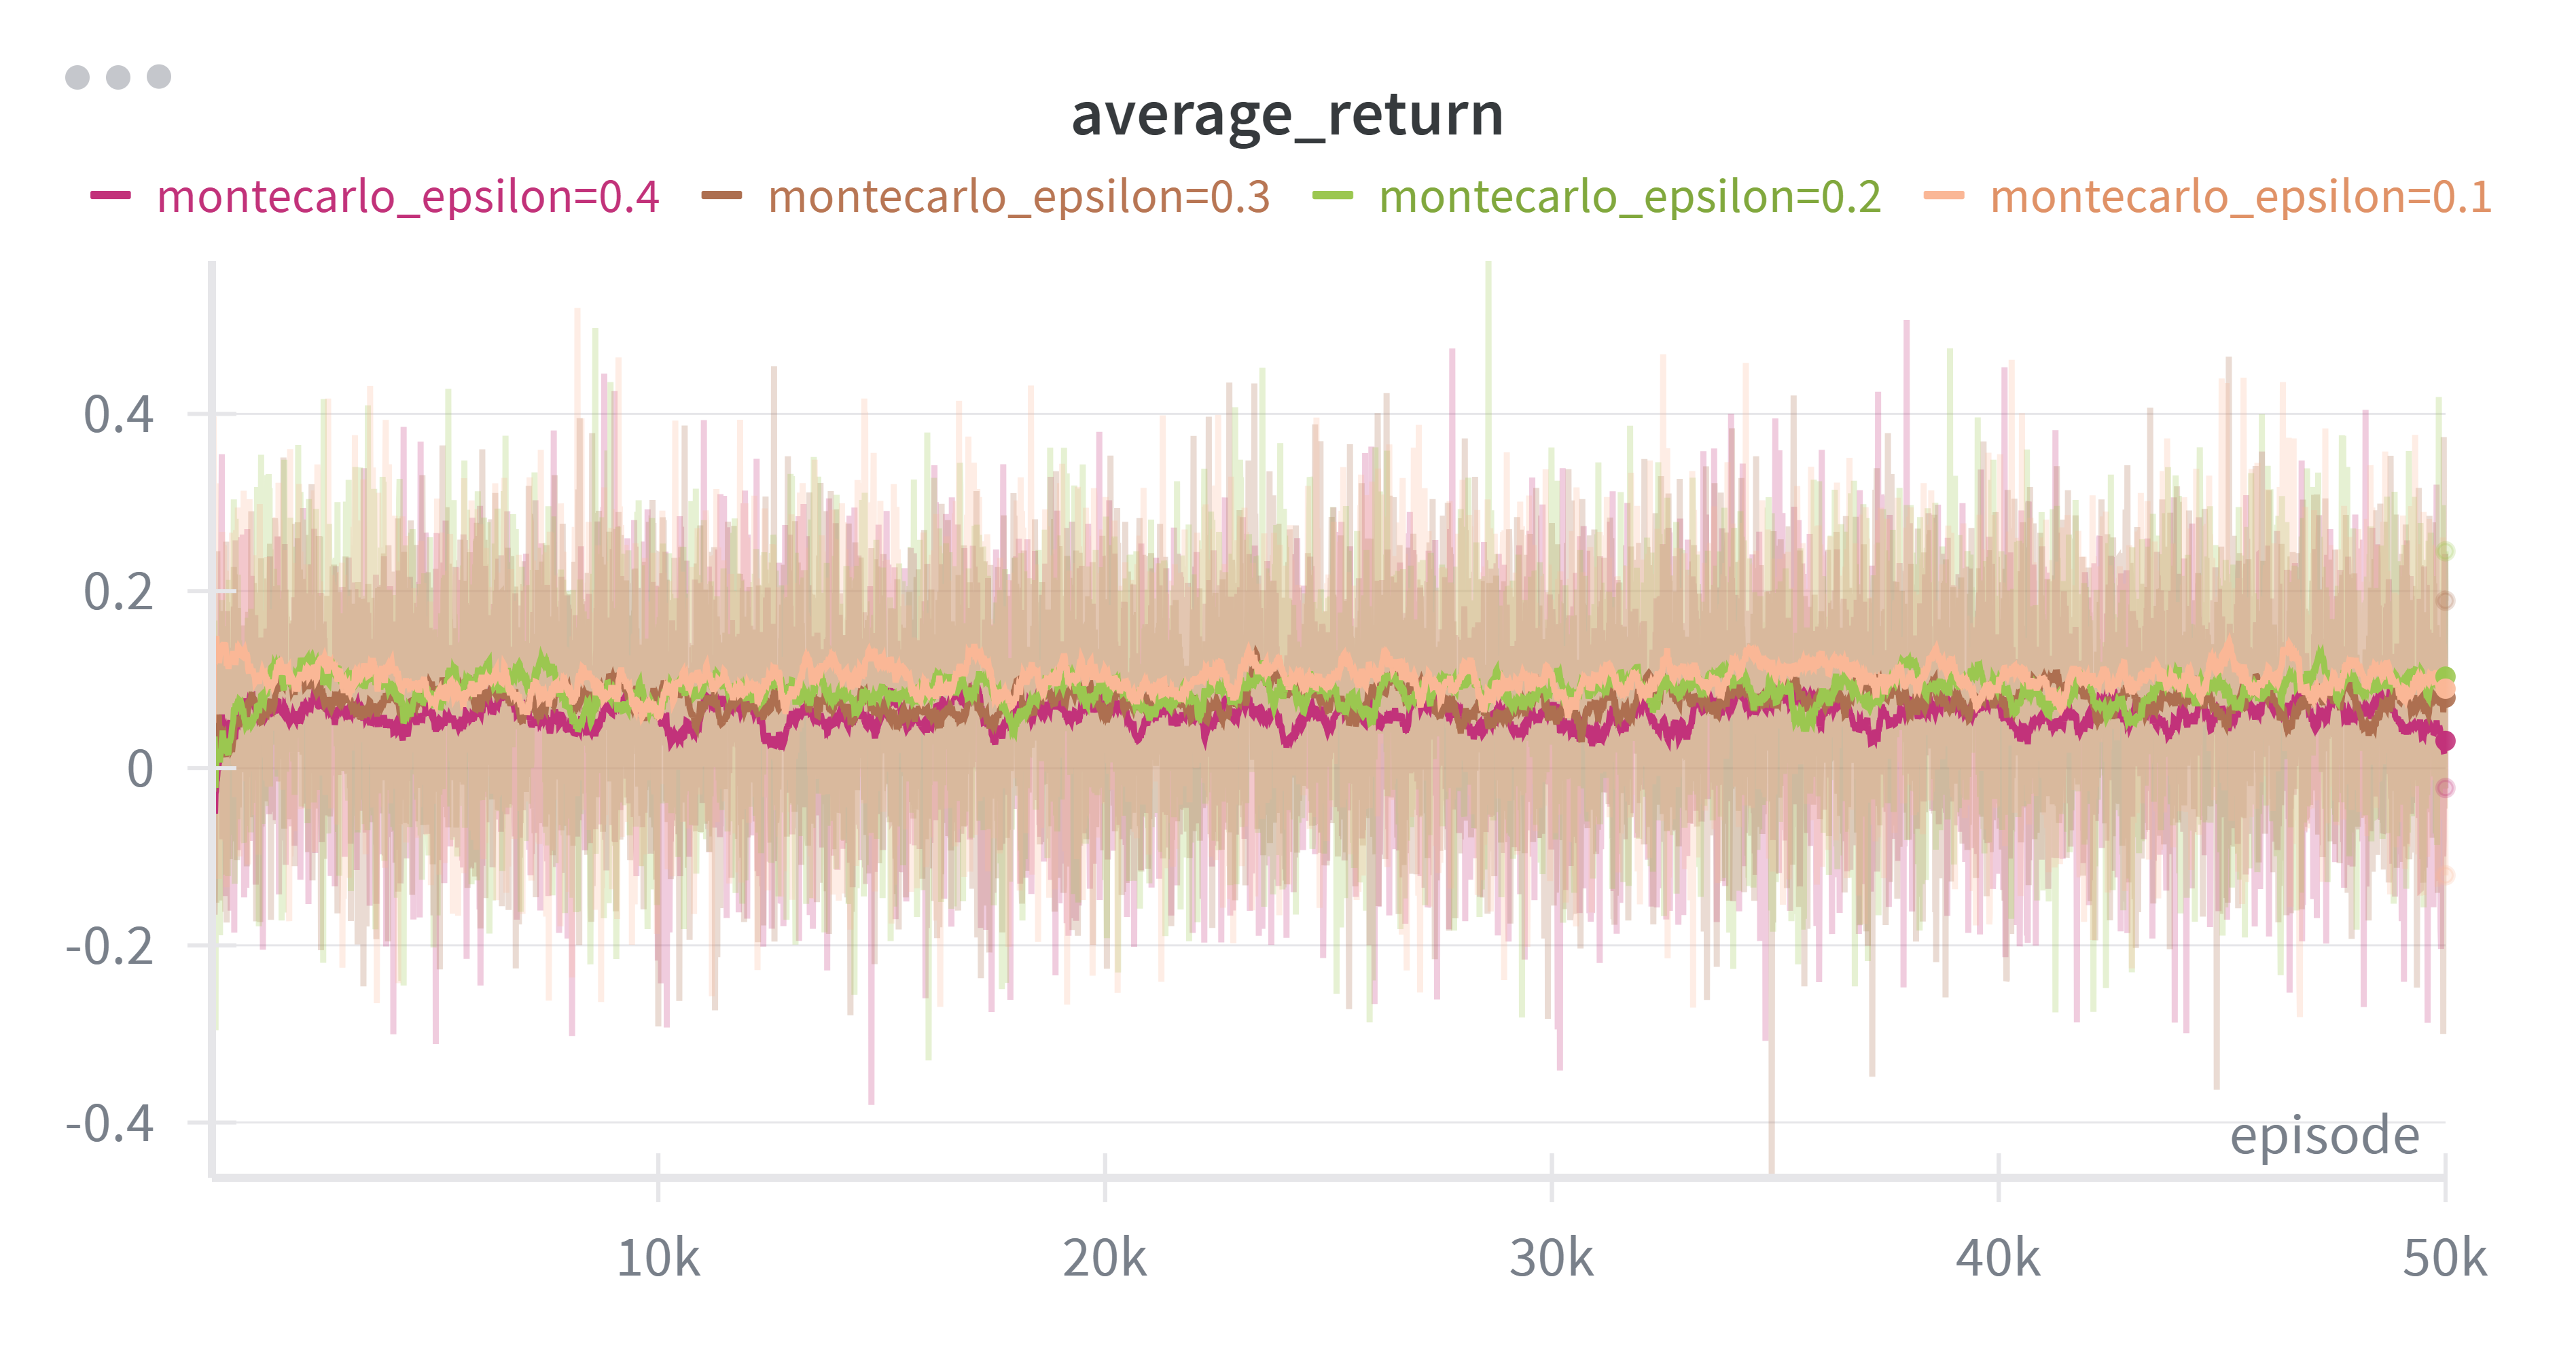
\includegraphics[width=0.5\textwidth]{Myimages/montecarlo_return.png}
            \caption{Monte Carlo Learning Curve}
            \label{fig:montecarlo learning curve}
        \end{figure}
        \begin{figure}[H]
            \centering
            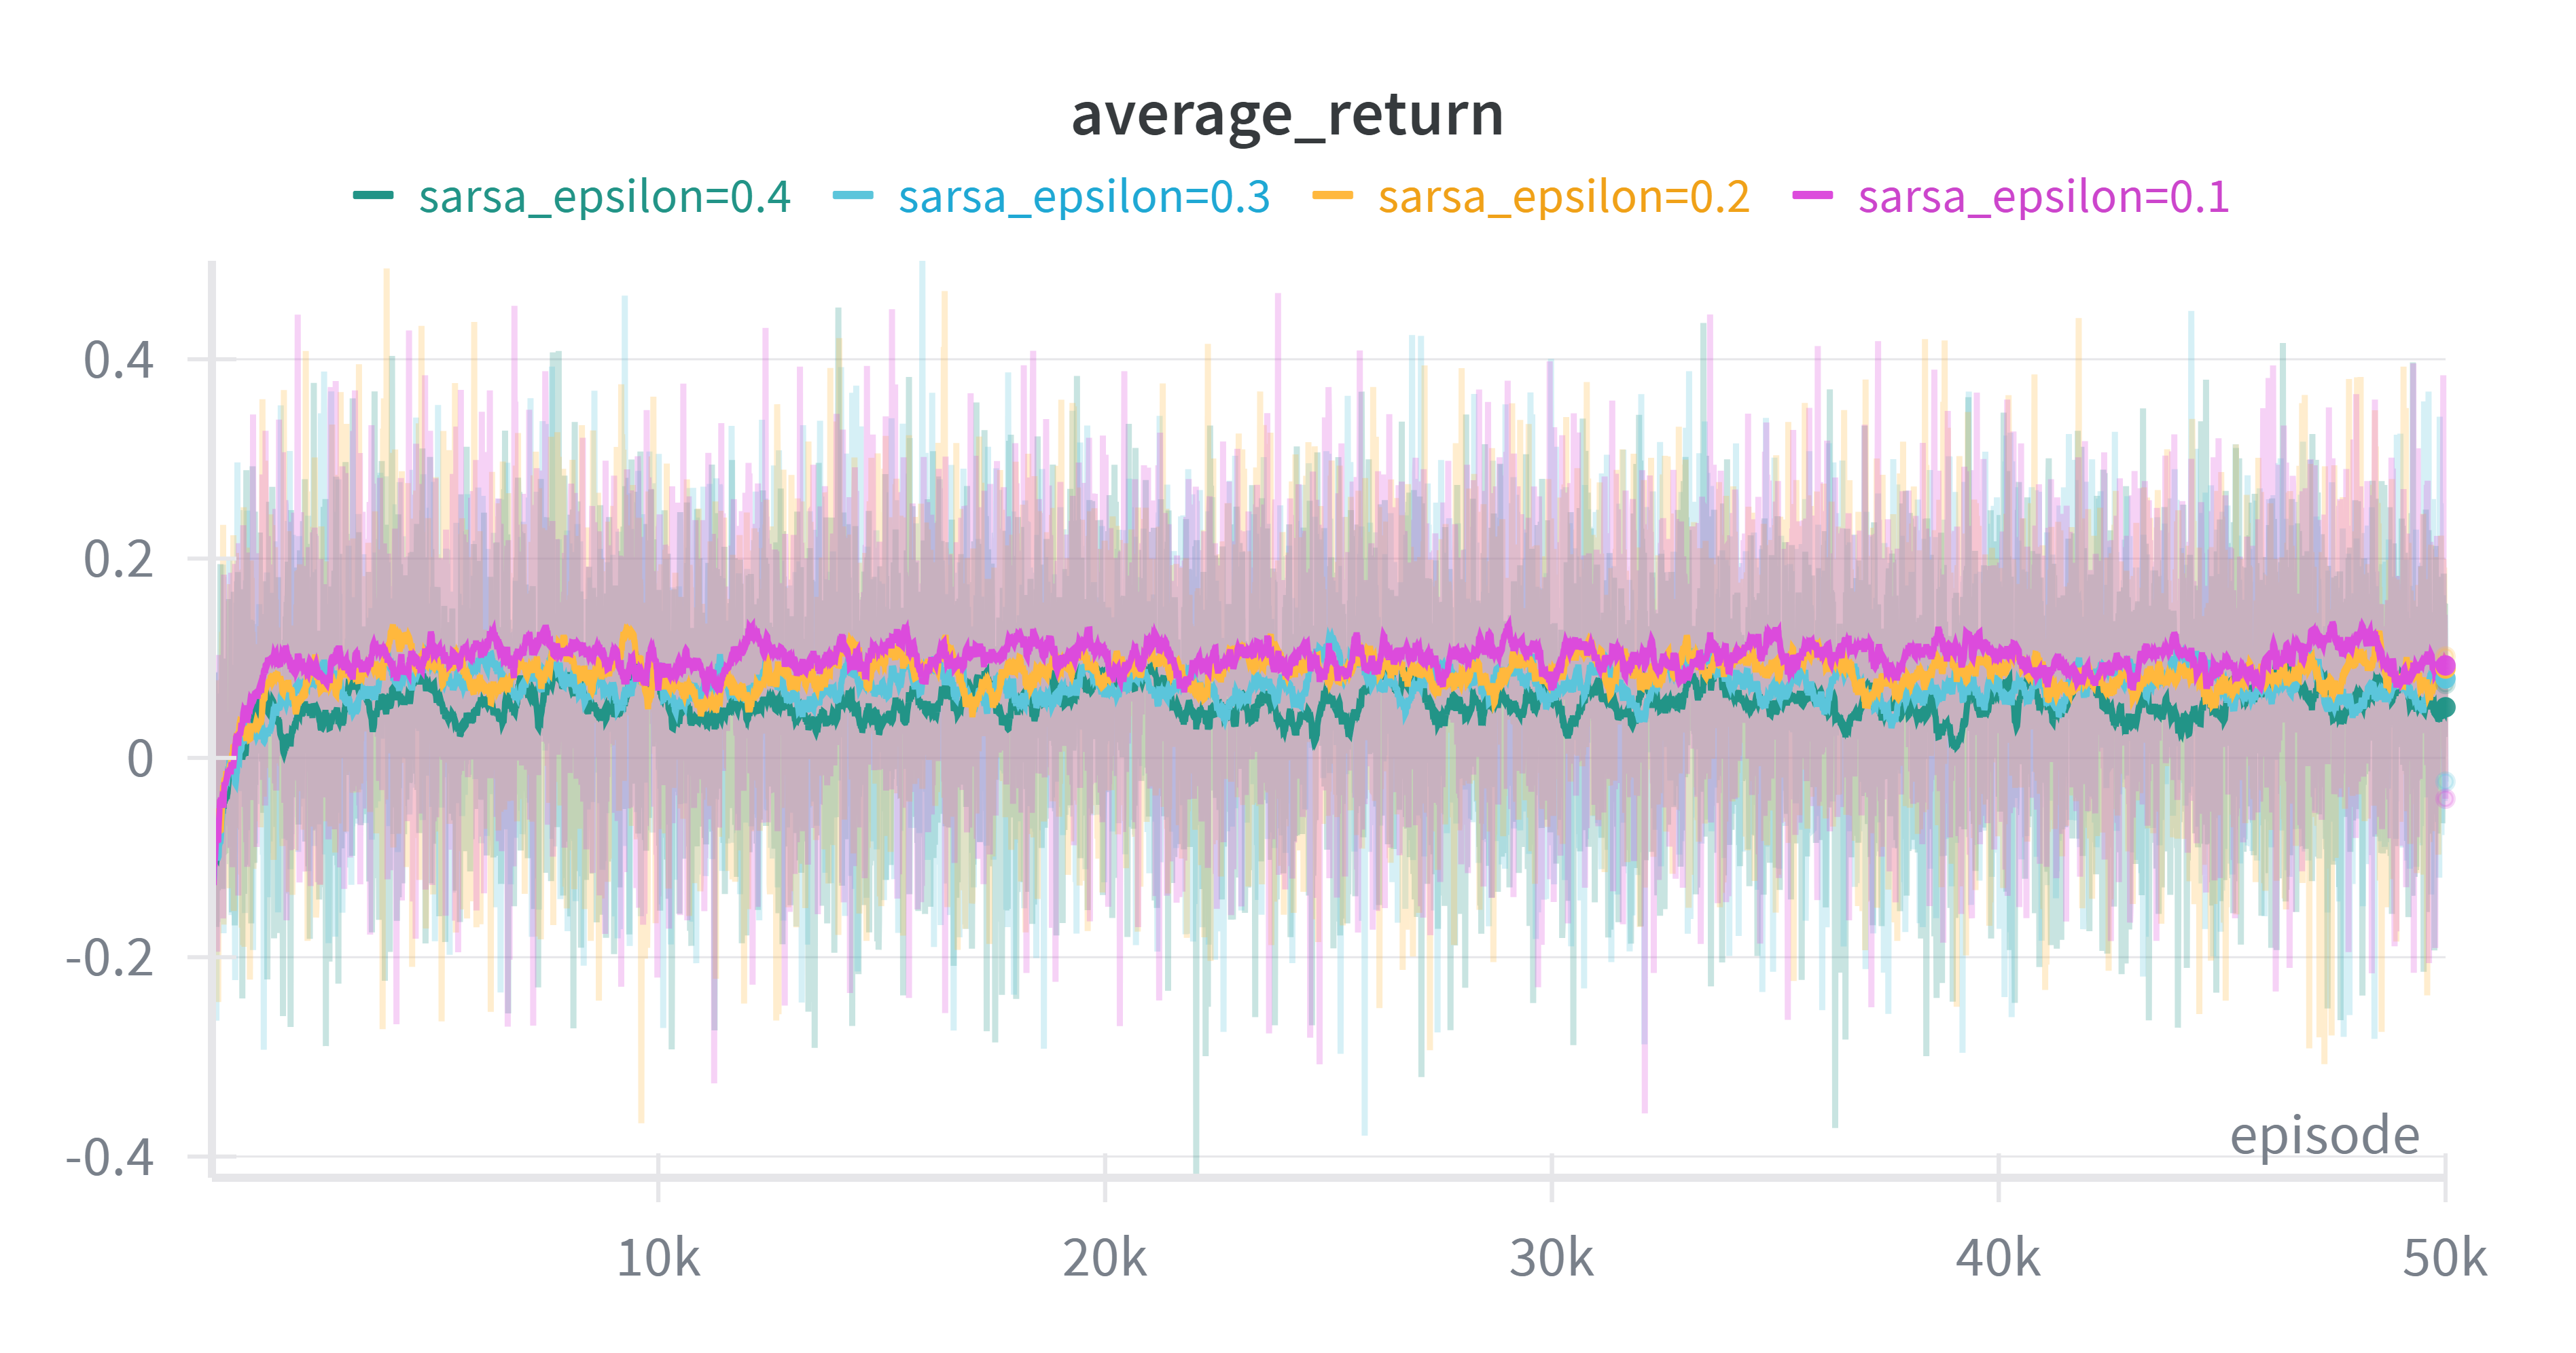
\includegraphics[width=0.5\textwidth]{Myimages/sarsa_return.png}
            \caption{SARSA Learning Curve}
            \label{fig:sarsa learning curve}
        \end{figure}
        \begin{figure}[H]
            \centering
            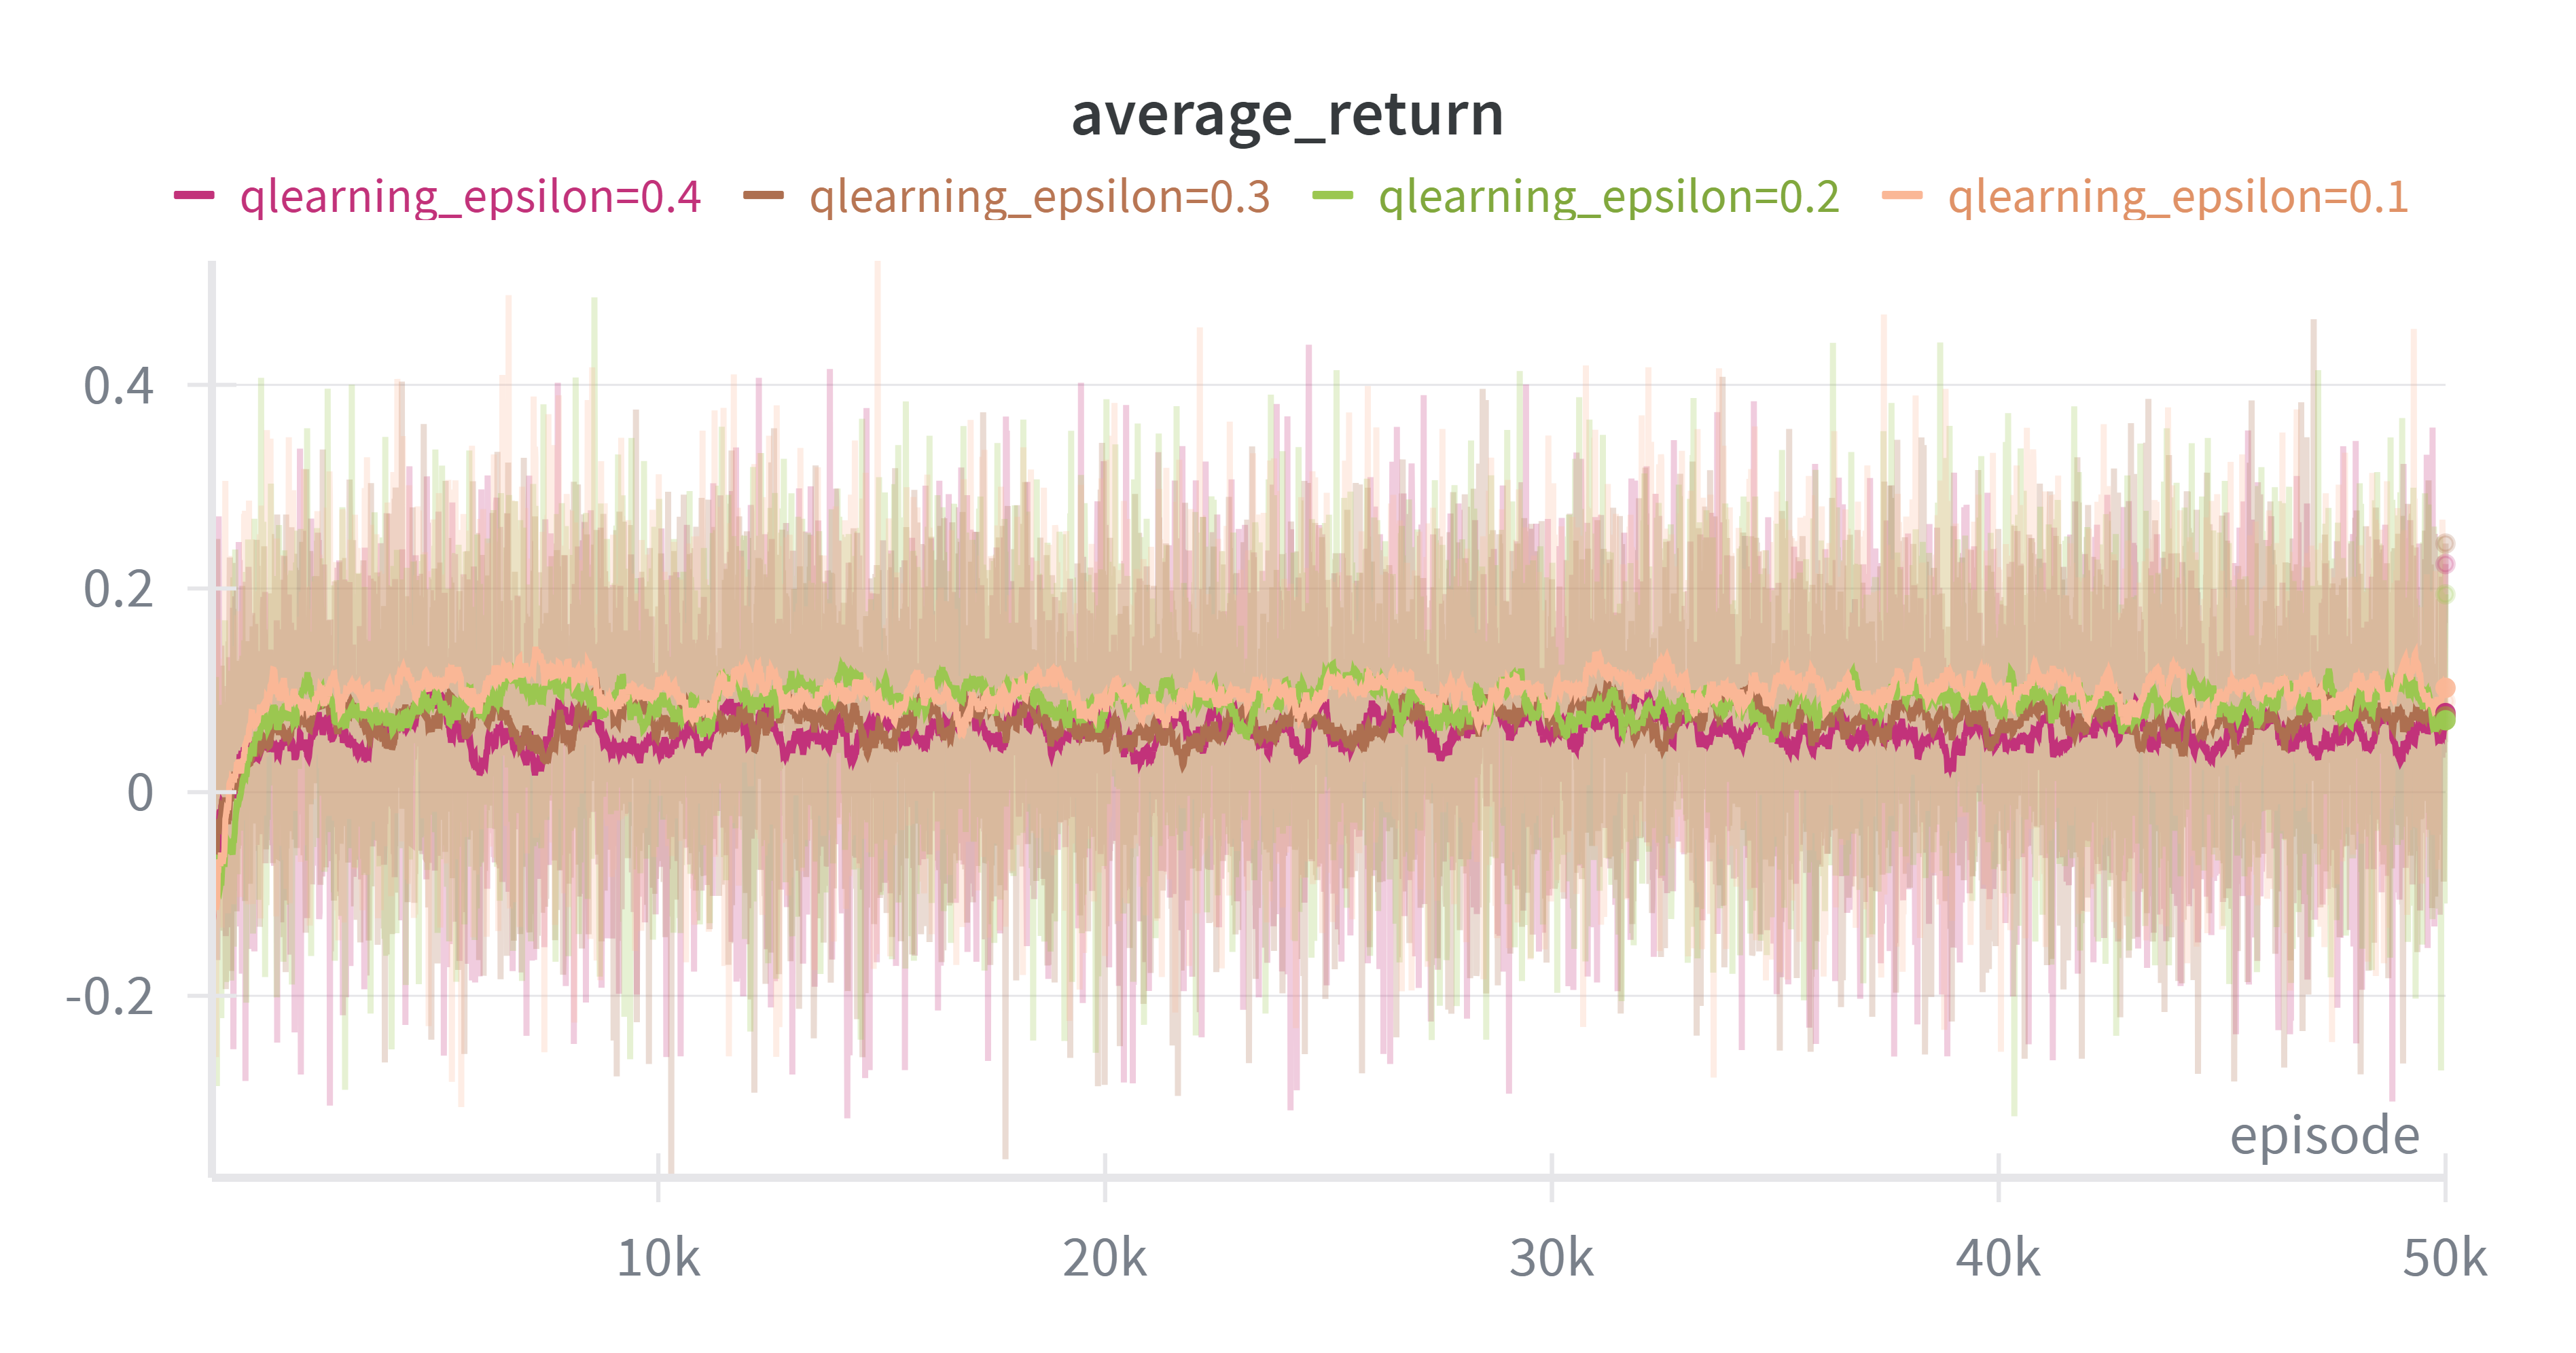
\includegraphics[width=0.5\textwidth]{Myimages/qlearning_return.png}
            \caption{Q-Learning Learning Curve}
            \label{fig:qlearning learning curve}
        \end{figure}
        \begin{figure}[H]
            \centering
            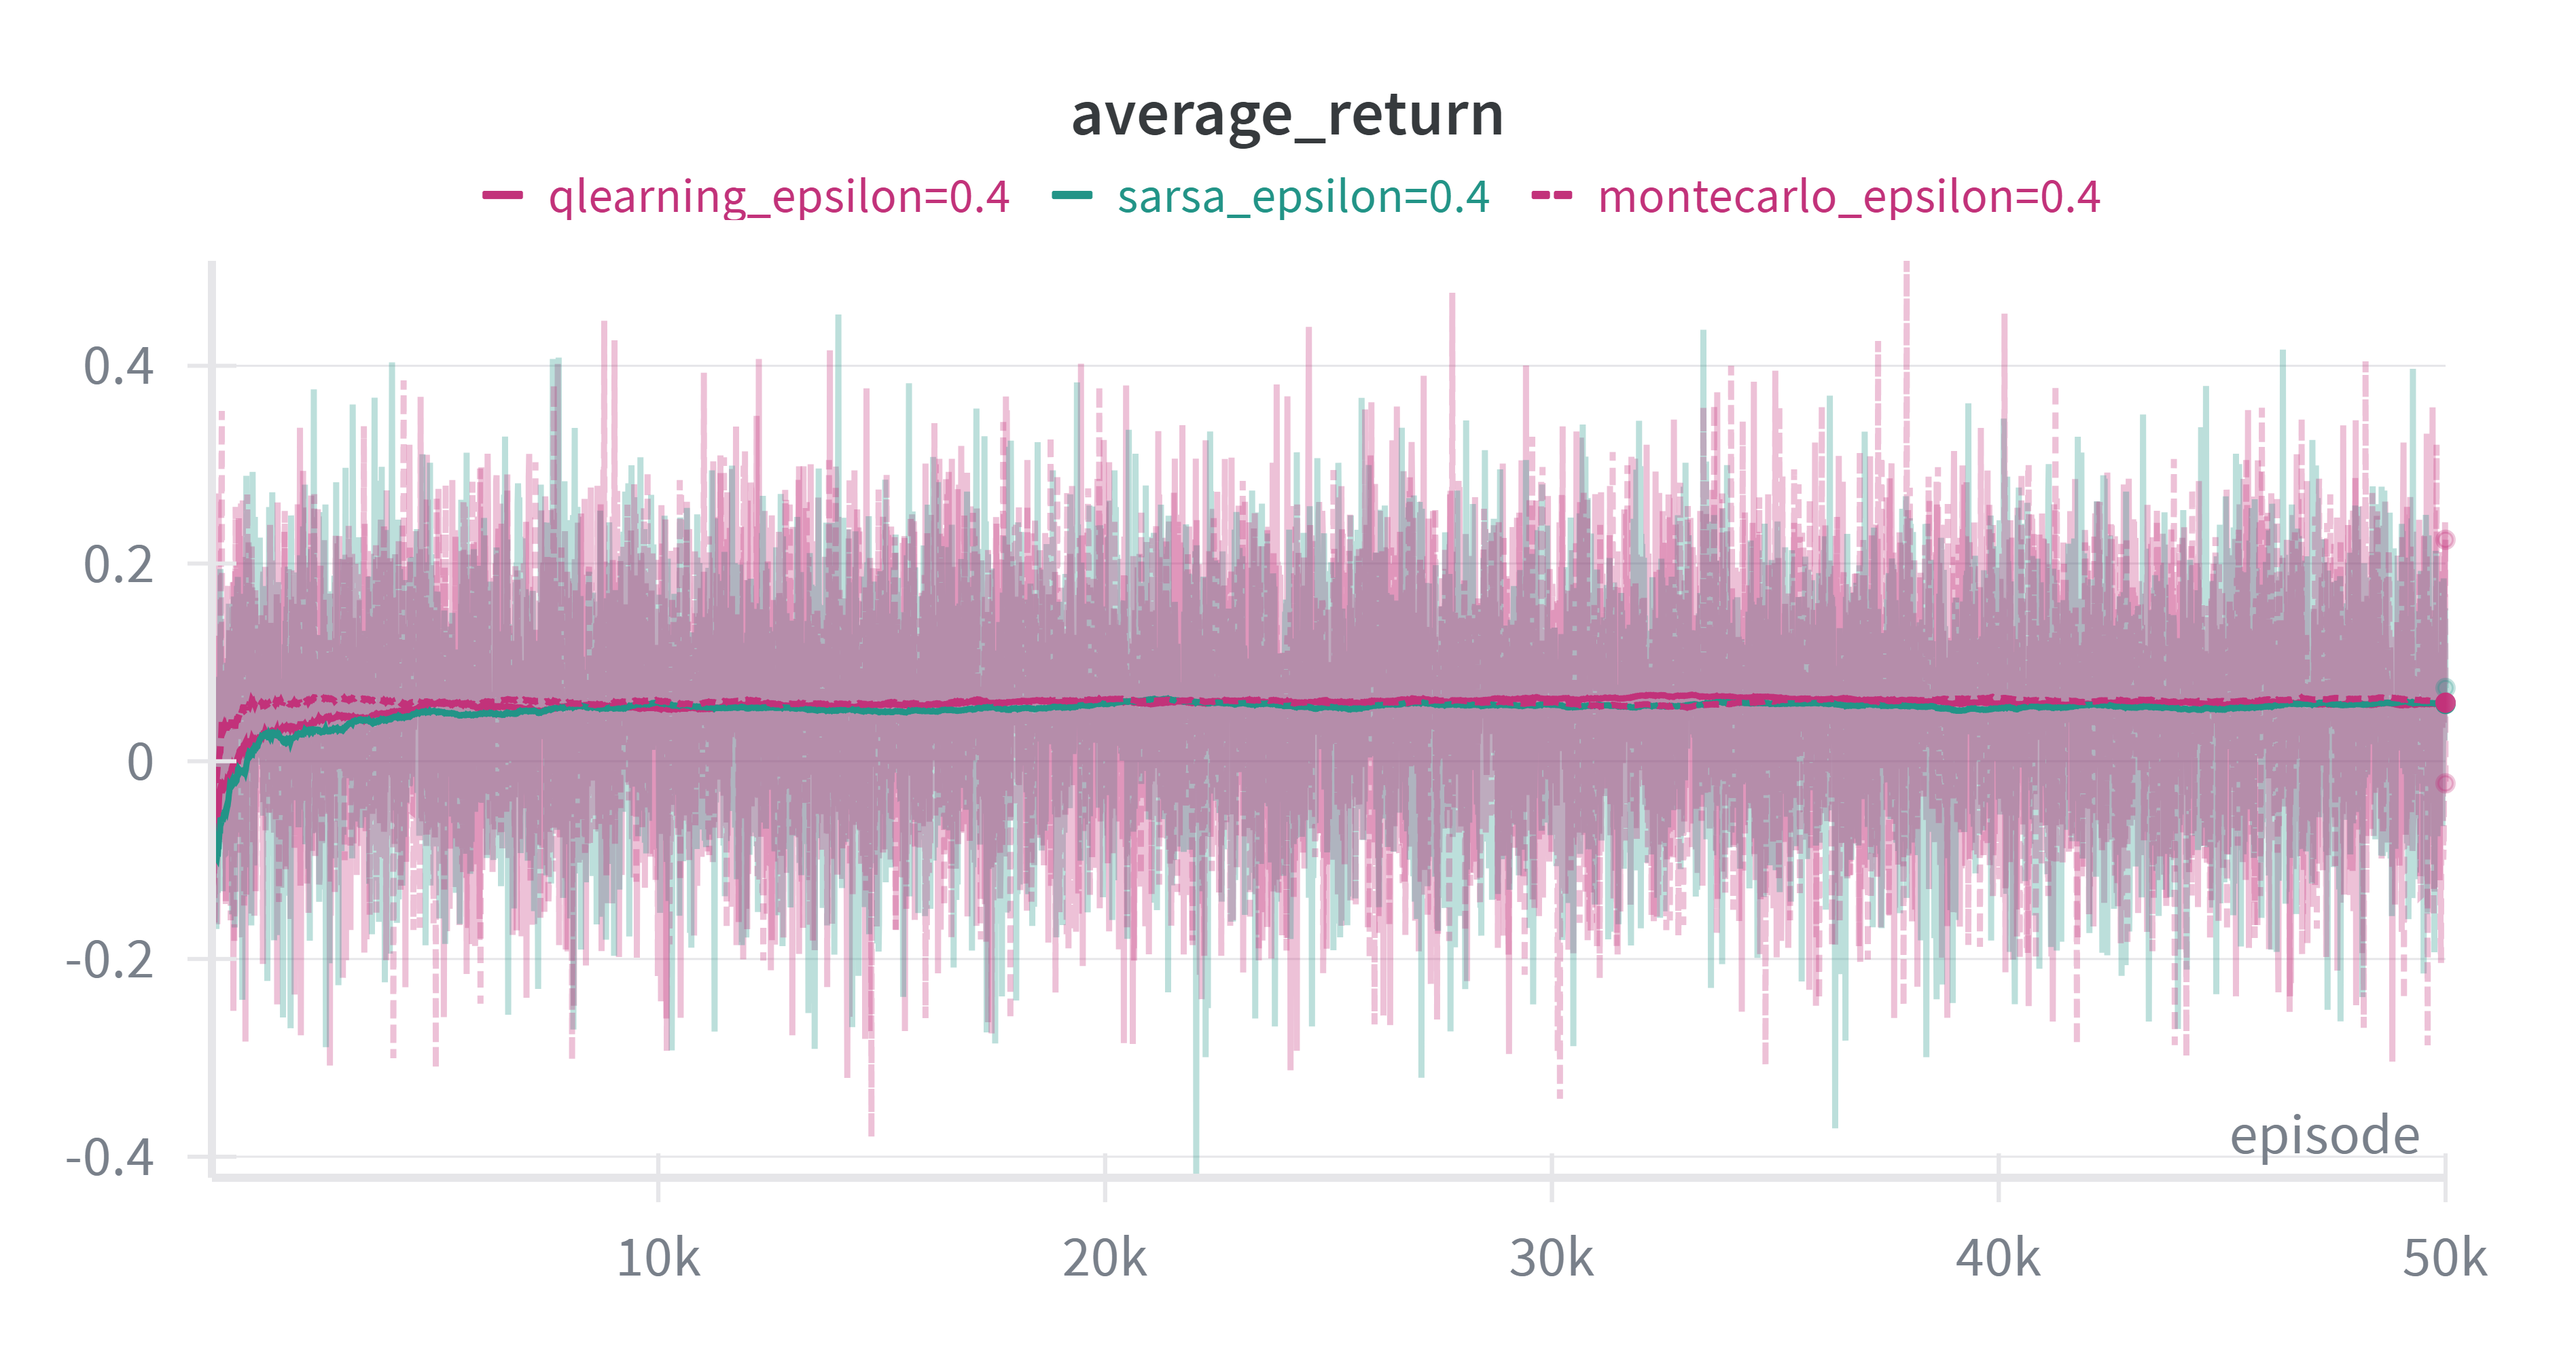
\includegraphics[width=0.5\textwidth]{Myimages/return_between_methods.png}
            \caption{Return Comparison Between Methods}
            \label{fig:return between methods}
        \end{figure}
        \textbf{Analysis:} \\
            \begin{enumerate}
                \item \textbf{Early Exploration:} Typically, a higher $\epsilon$ value leads to more exploration in the early stages of learning. And the 
                convergence speed would be faster since the agent is more likely to explore different actions and states.
                What is worth noting is that Monte-Carlo converge slightly faster in the early stages, This is likely because the full return provides a more accurate estimate of the value function.
            \end{enumerate}
                \item \textbf{Convergence value between ($\epsilon$):} Clearly, a lower $\epsilon$ value leads to a higher convergence value. This is because a lower $\epsilon$ produces a more deterministic policy in the long run,
                which allows the agent to exploit the learned value function more effectively. 
                \item \textbf{Convergence value between methods:} In my experiments, I found that all three methods have similar trends and the same convergence value. This likely results from the simple
                environment, where a nearly optimal policy can be learned quickly. In a more complex environment, differences between methods may appear if the max\_episodes are not sufficient
                for the agent to learn the optimal policy.
                
        

    \end{answer}

    \begin{answer}[Q3. Discuss and plot loss curves under $\epsilon$ values of $(0.1, 0.2, 0.3, 0.4)$ on MC, SARSA, and Q-Learning]
        \textbf{Description:} \\
        During this session, I implemented Monte-Carlo, SARSA, and Q-Learning for control tasks. I ran the experiments for over 4 different $\epsilon$ values
        and compared the loss curves. The loss curves are shown in the figures below.
        \begin{figure}[H]
            \centering
            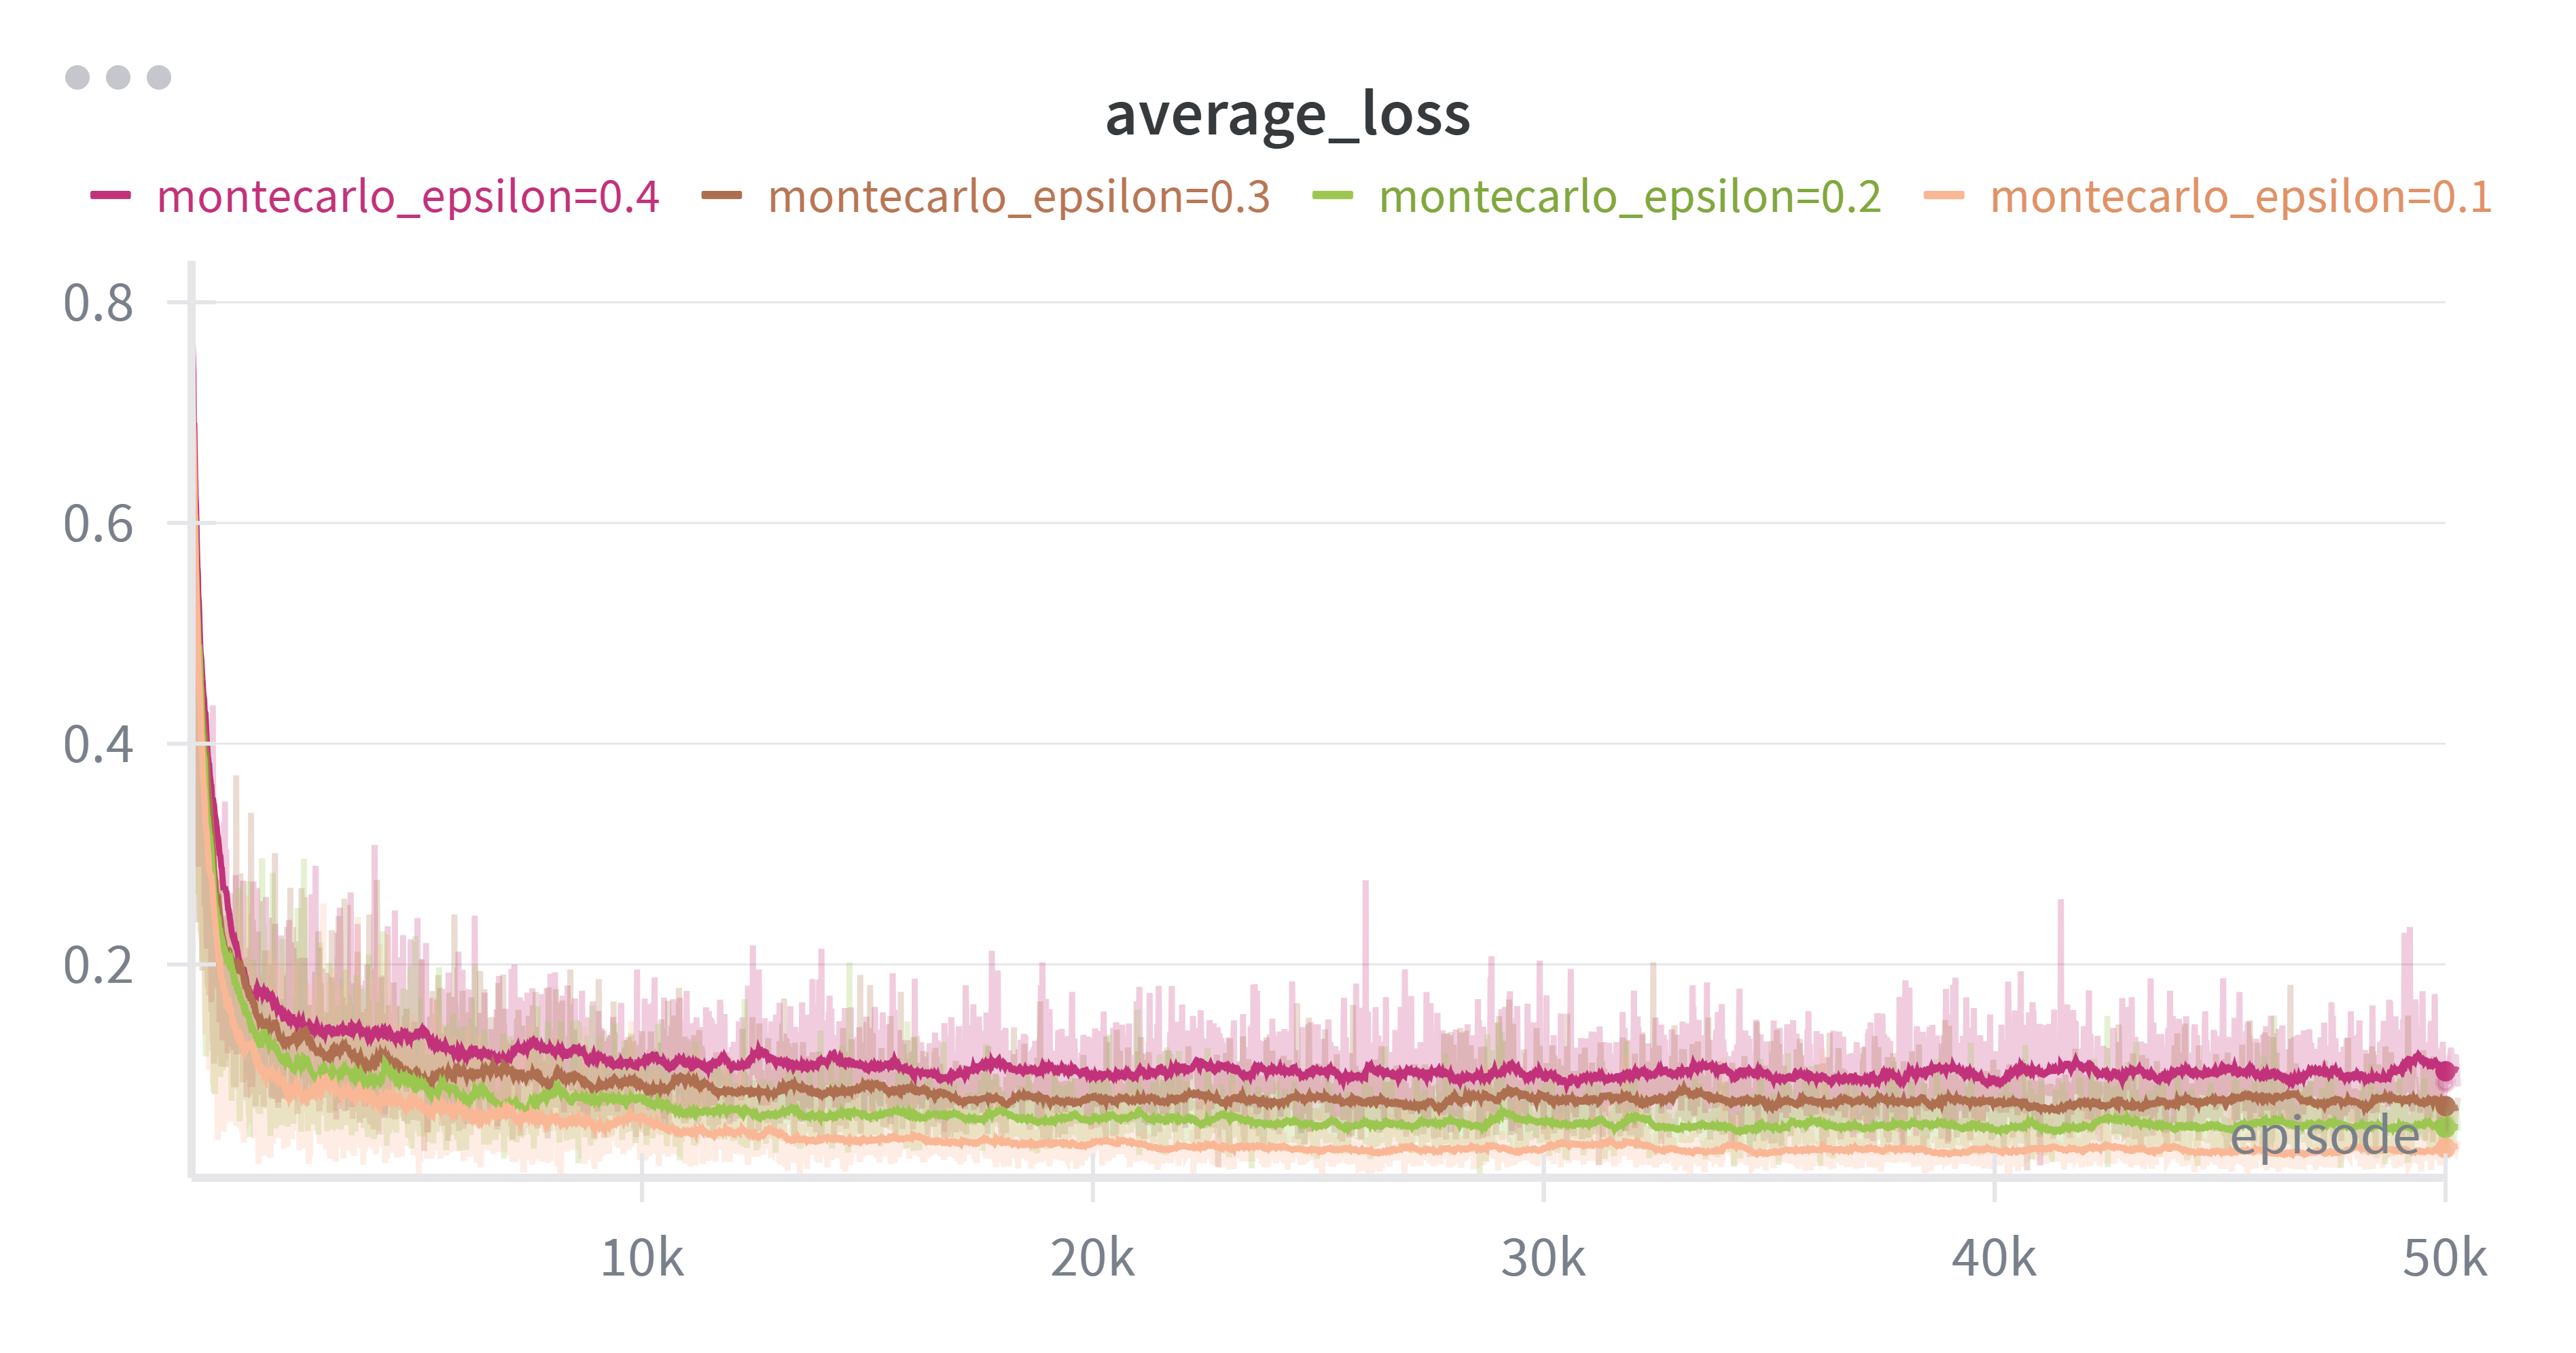
\includegraphics[width=0.5\textwidth]{Myimages/montecarlo_loss.png}
            \caption{Monte Carlo Loss Curve}
            \label{fig:montecarlo loss curve}
        \end{figure}
        \begin{figure}[H]
            \centering
            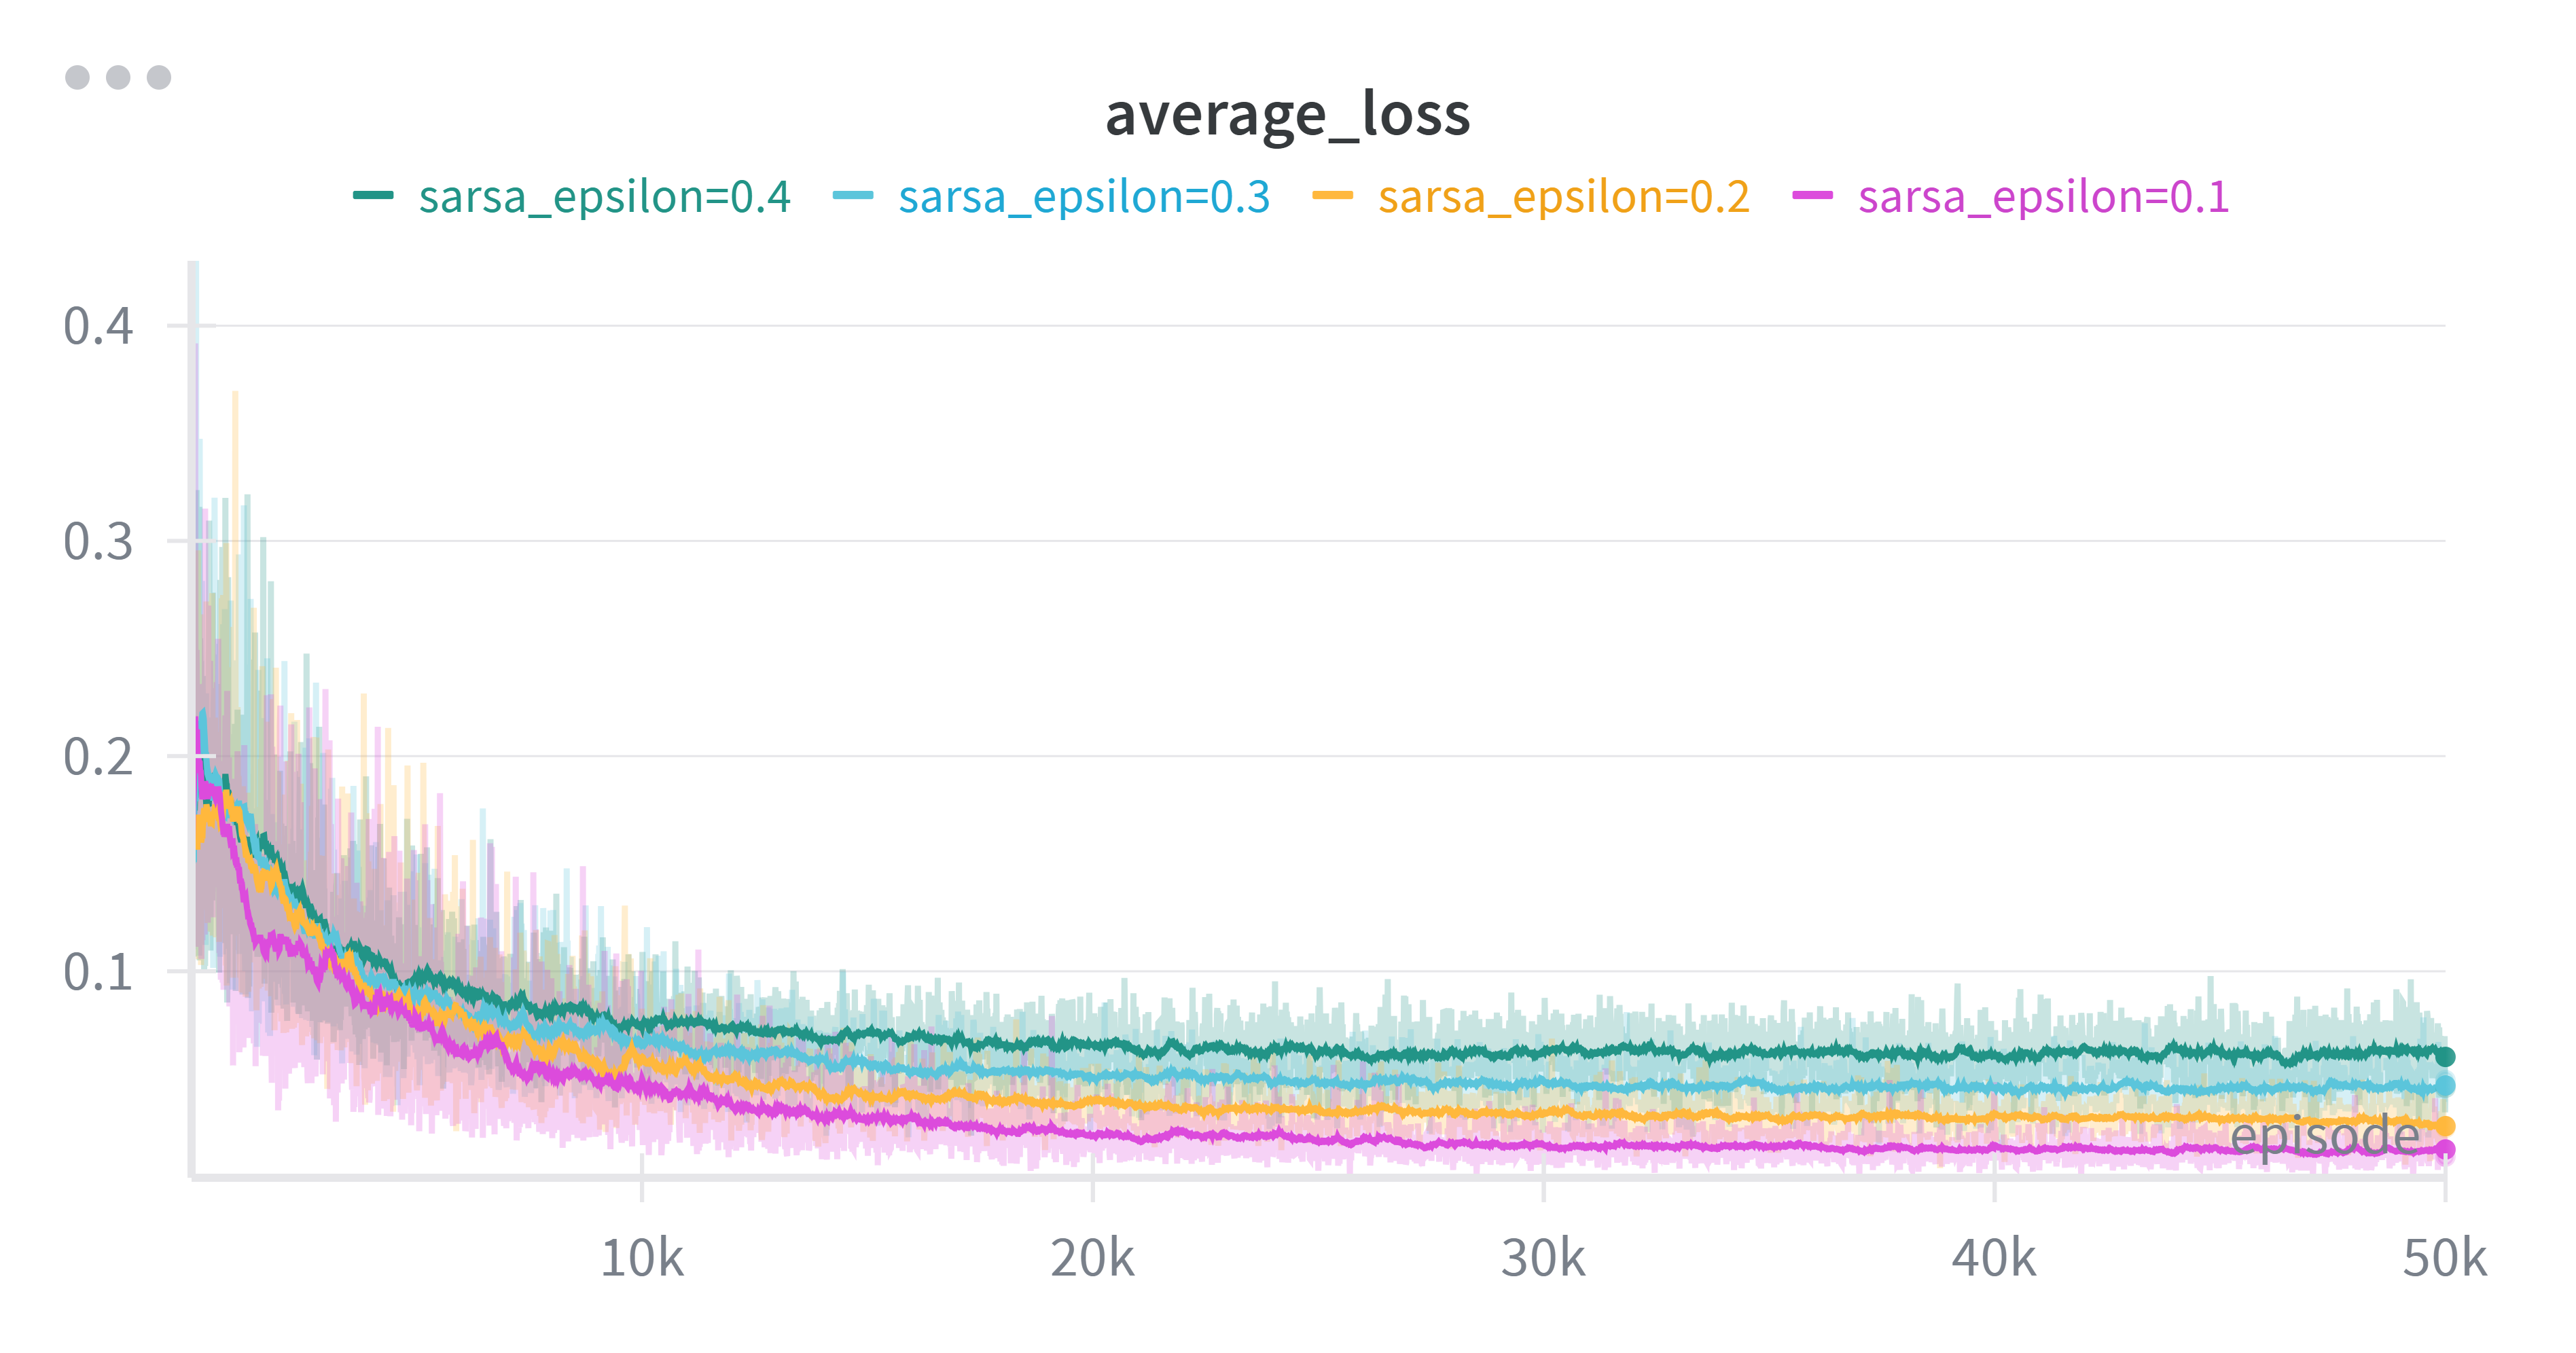
\includegraphics[width=0.5\textwidth]{Myimages/sarsa_loss.png}
            \caption{SARSA Loss Curve}
            \label{fig:sarsa loss curve}
        \end{figure}
        \begin{figure}[H]
            \centering
            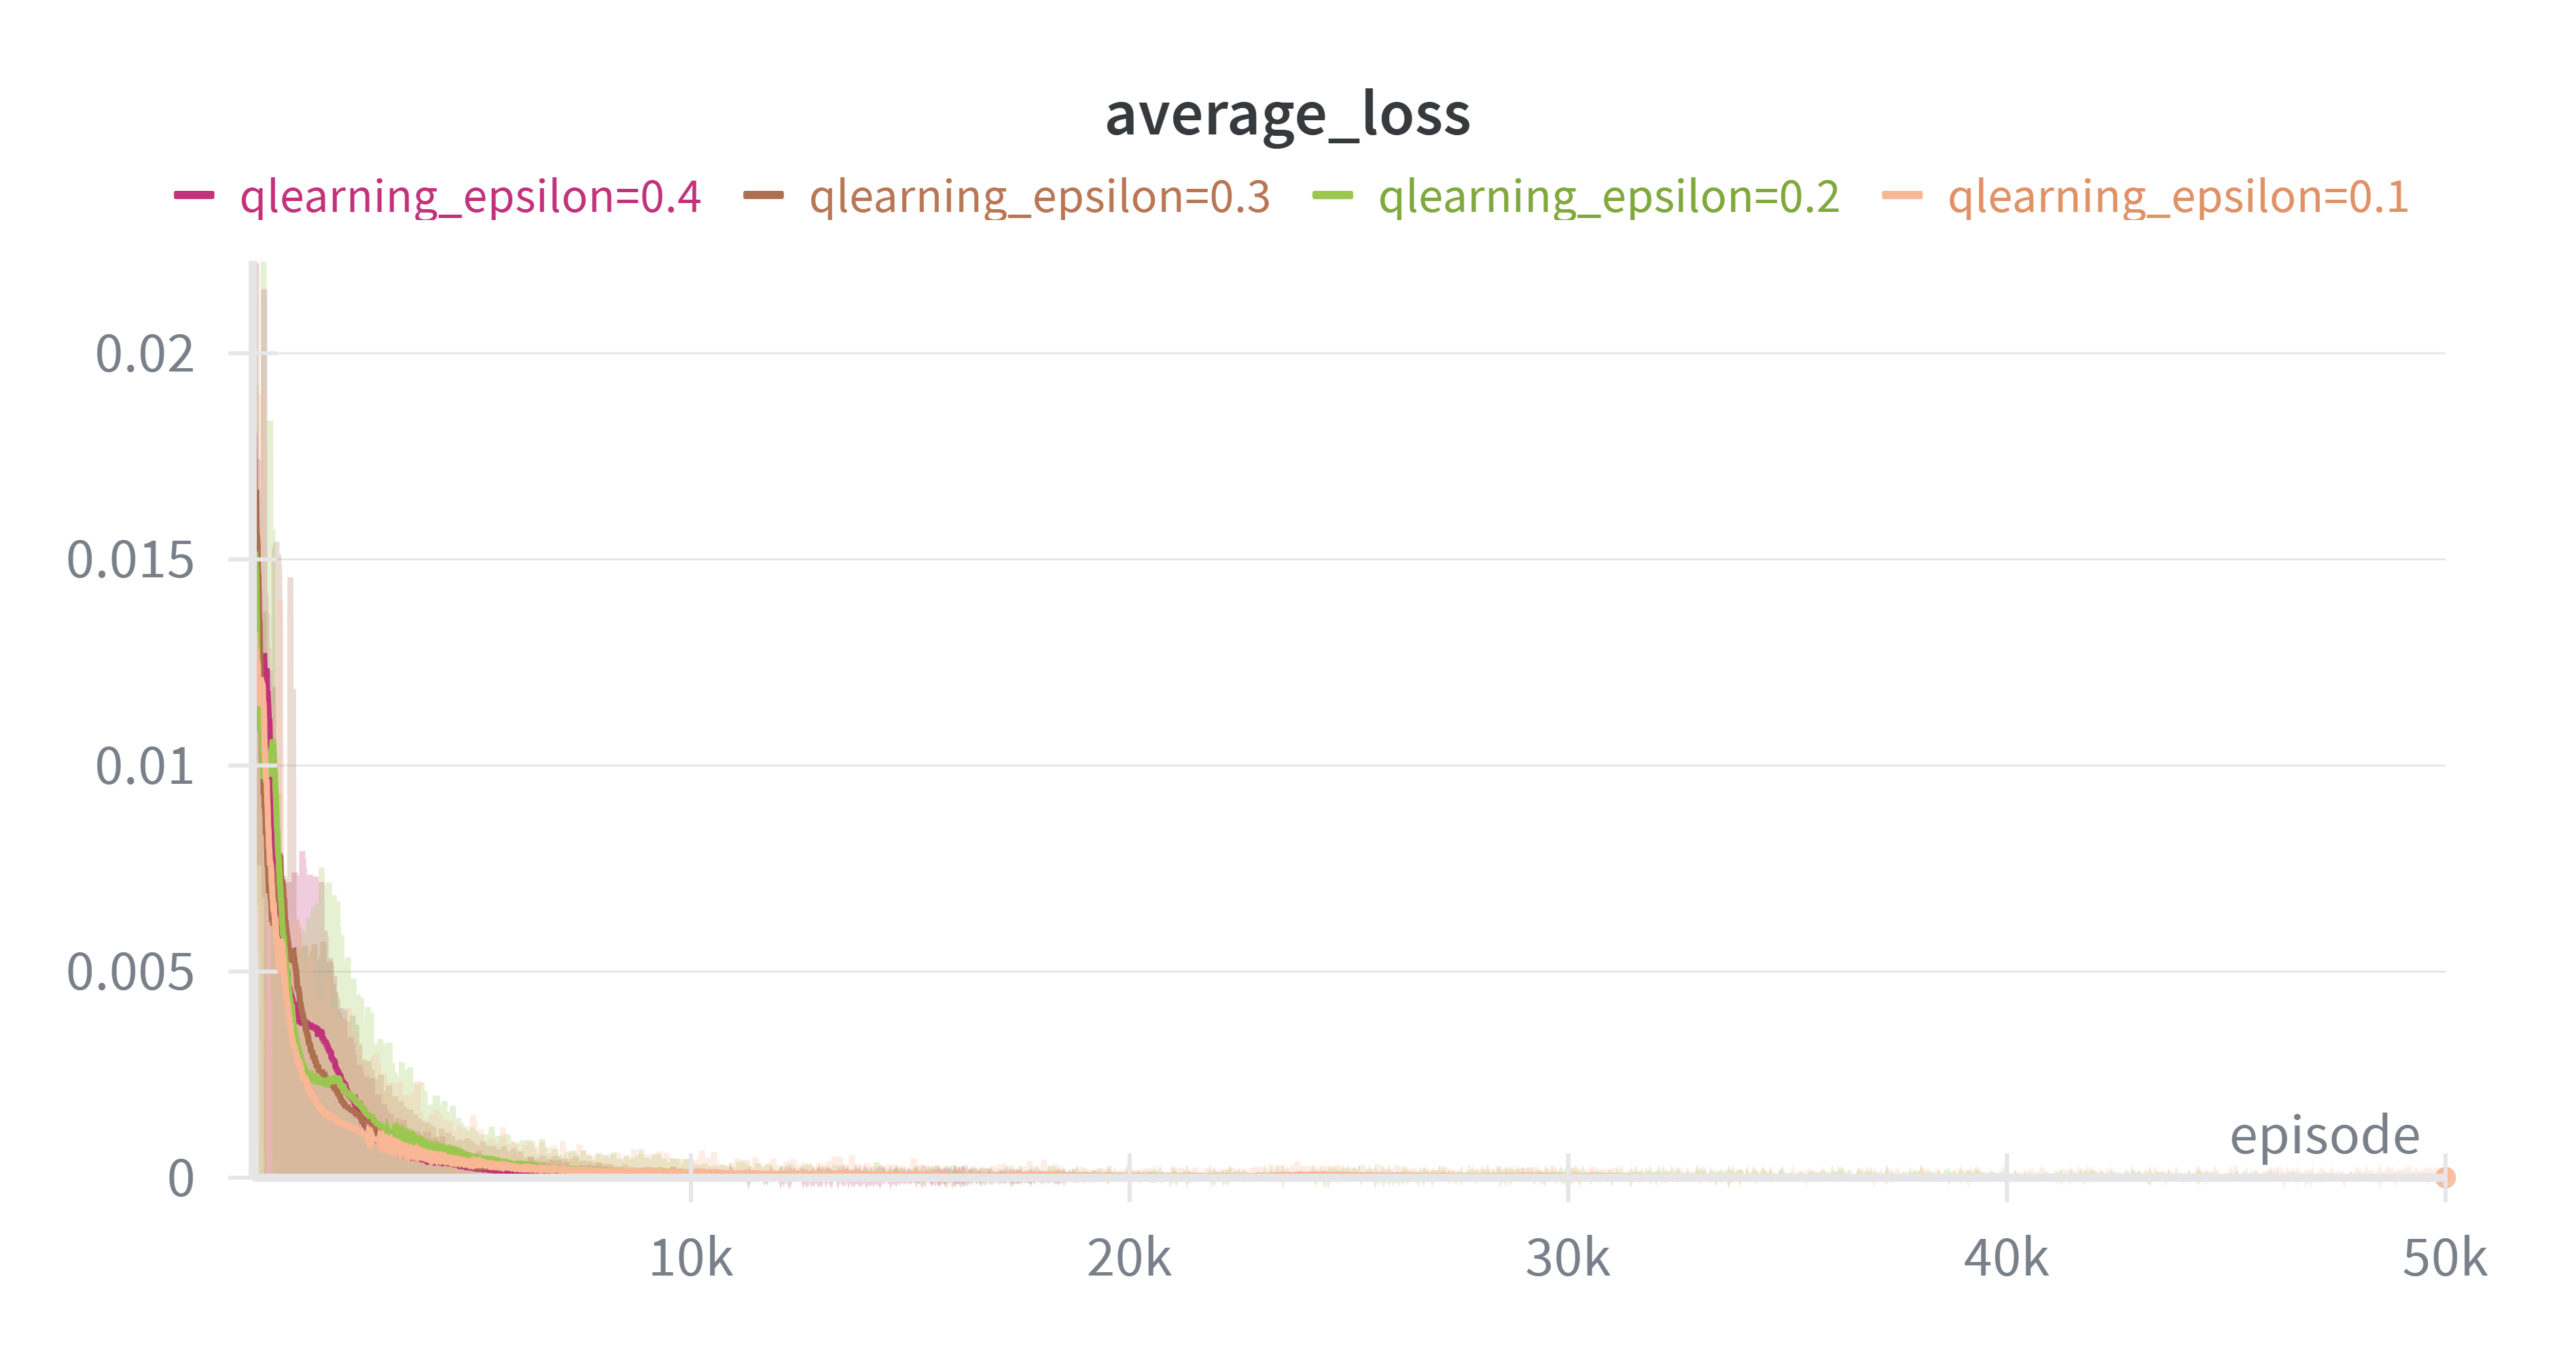
\includegraphics[width=0.5\textwidth]{Myimages/qlearning_loss.png}
            \caption{Q-Learning Loss Curve}
            \label{fig:qlearning loss curve}
        \end{figure}
            \begin{figure}[H]
                \centering
                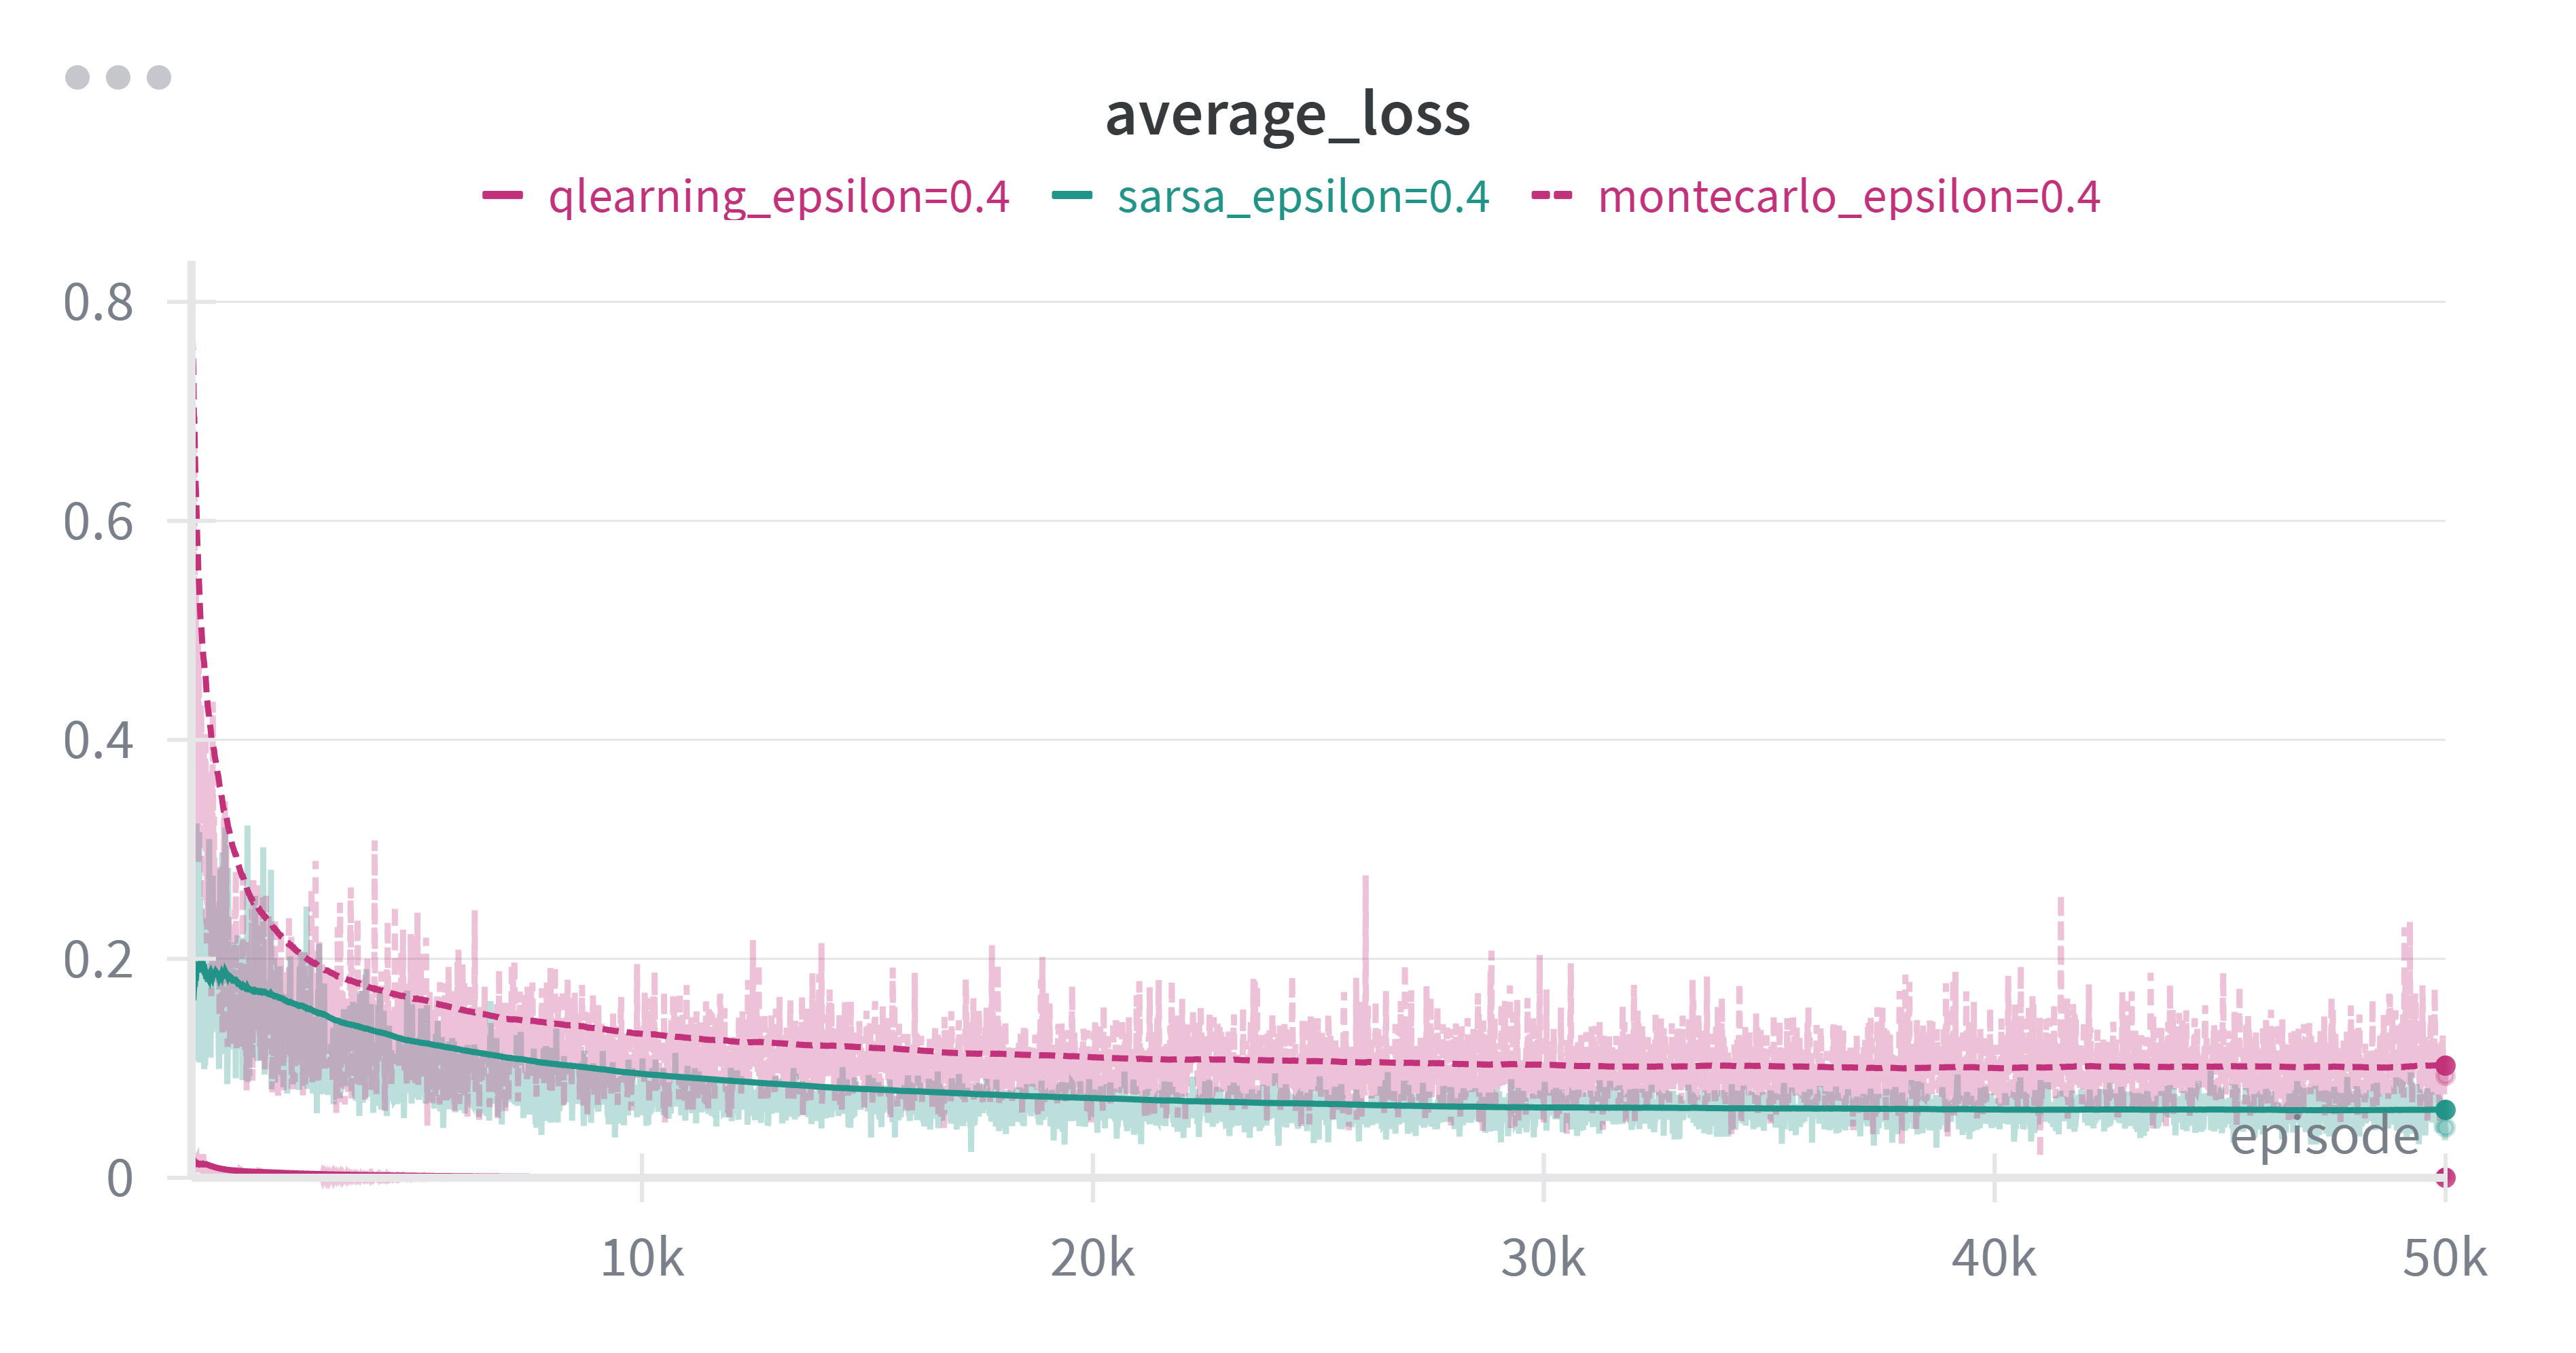
\includegraphics[width=0.5\textwidth]{Myimages/loss_between_methods.png}
                \caption{Loss Comparison Between Methods}
                \label{fig:loss between methods}
            \end{figure}
        \textbf{Analysis:} \\
        \begin{enumerate}
            \item \textbf{Loss trends:} In general, all three methods show that the loss decreases quite fast in the early stages, 
            and becomes flatter as the episodes increase. 
            \item \textbf{Comparison between $\epsilon$:} like the return curves, a higher $\epsilon$ value leads to higher loss in the long run 
            since the agent's action is more random, making the loss larger due to the increased uncertainty.
            \item \textbf{Comparison Between Methods:} In general, q-learning has the smallest loss among the three methods. This stems from the loss design, we always use the max action to calculate the loss, 
            which leads to a smaller loss. SARSA has a higher loss since it uses the action from the epsilon-greedy policy to calculate the loss, which may not the optimal action.
            As for Monte-Carlo, it has the highest loss since it uses the full return to calculate the loss, which includes all the randomness in the episode.
        \end{enumerate}

    \end{answer}
\end{document}